%! TEX root = ../thesis.tex

\chapter{Extensive air showers}
\label{chapter:extensive-air-showers}

Consider a high energy cosmic ray impinging on earth. The questions pertaining to where it might originate from and how it has gained so much kinetic energy have 
been answered in the preceding sections. In the following, the particle cascades resulting from the particle interacting in the upper atmosphere will be examined. 
This is done in a two-fold way. The underlaying principles will be explained via considering a particle carrying no SU$(3)$-color charge in 
\autoref{sec:heitler-model}. The more general treatment for hadronic showers is then found in \autoref{sec:heitler-matthews-model}. As supplementary information, 
the effect of different hadronic primaries is discussed in \autoref{sec:superposition-principle}.

\section{Electromagnetic showers}
\label{sec:heitler-model}

\begin{figure}
	\begin{subfigure}[b]{0.425\textwidth}
		\centering
		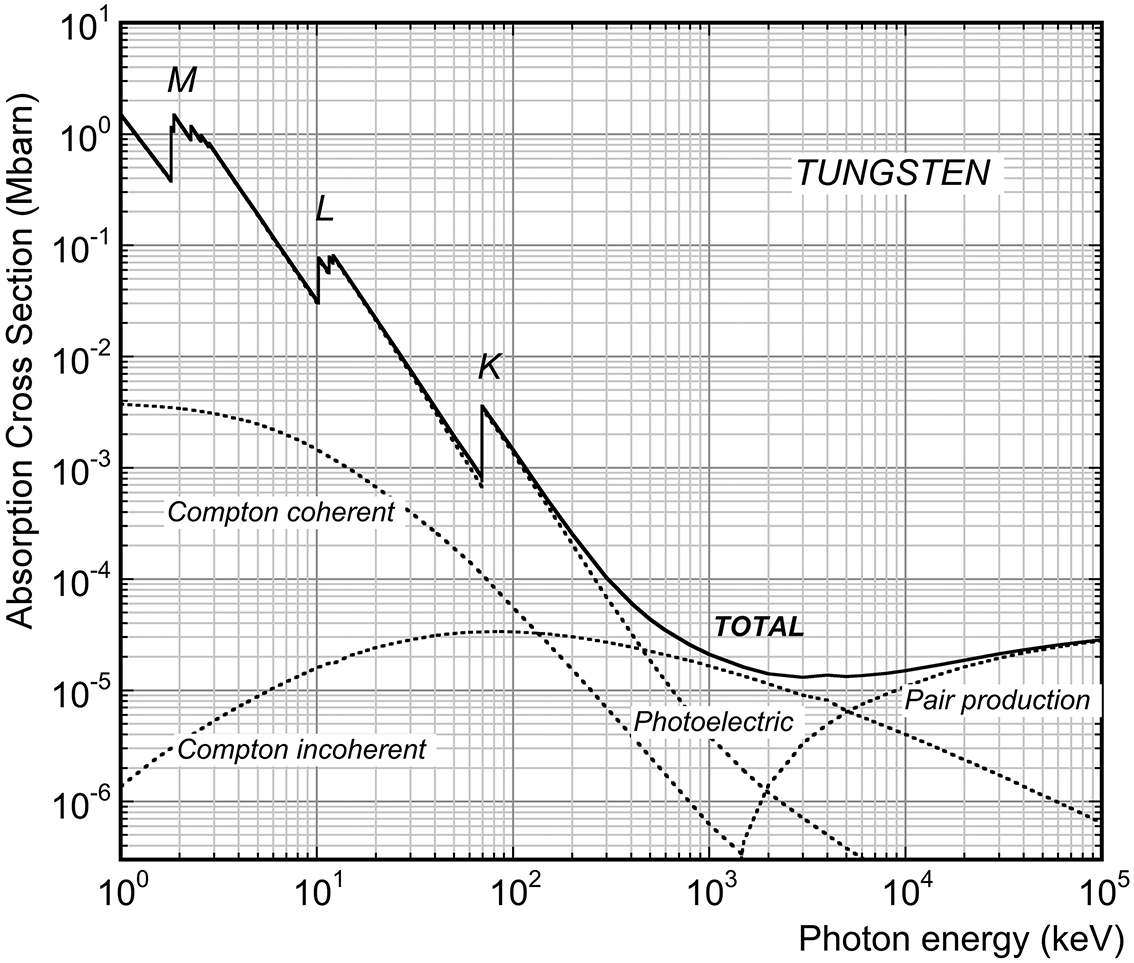
\includegraphics[width=\textwidth]{./plots/photon_cross_section.png}
		\caption{$\mathbf{\gamma}$\textbf{ interactions}}
		\label{fig:gamma-interactions}
	\end{subfigure}
	\hfill
	\begin{subfigure}[b]{0.575\textwidth}
		\centering
		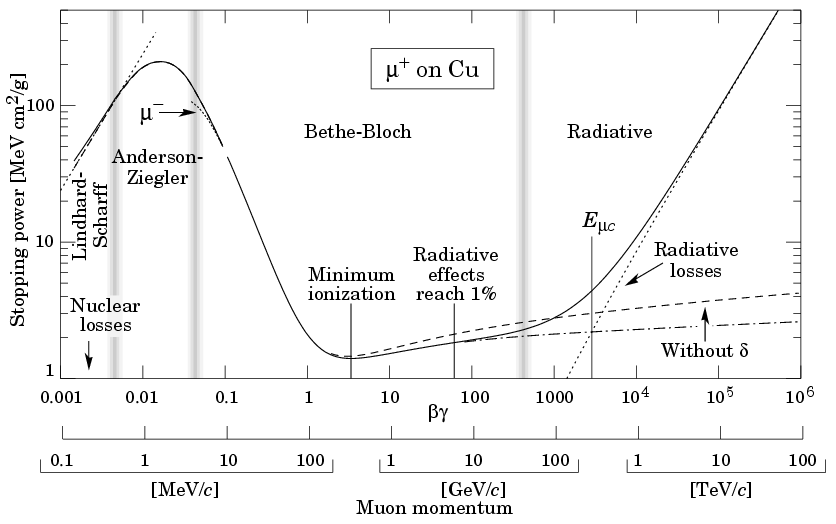
\includegraphics[width=\textwidth]{./plots/electron_ionisation_loss.png}
		\caption{$\mathbf{e^\pm}$\textbf{ interactions}}
		\label{fig:electron-interactions}
	\end{subfigure}
	\caption{\textbf{(a)} Cross section for different energy loss processes of a photon in tungsten. The sudden spikes correspond to the transition energy of 
	increasingly higher-energy electron shells. From \cite{chen2007interactions}. \textbf{(b)} Stopping power of copper, representatively on an antimuon $\upmu^+$, 
	with respect to its' momentum. Plot adopted with changes from \cite{meroli2017straggling}.}
	\label{fig:ionization-losses}
\end{figure}

The dominating interaction of $E > \SI{10}{\mega\electronvolt}$ photons in matter is $e^+e^-$ pair production, whereas for electrons/positrons the creation of a
$\gamma$ via bremsstrahlung prevails at high energies. This is shown in \autoref{fig:ionization-losses}. Consequently, an entire cascade of electrons, positrons 
and photons can emerge from a single primary particle, as realised by Heitler in \cite{heitler1984quantum}. 

Of particular interest in these showers are, apart from the primary particles energy $E_0$ and arrival direction $(\Upphi, \theta)$, the atmospheric depth 
$X_\text{max}$ at which it reaches its' maximum multiplicity, as well as the \textbf{L}ateral \textbf{D}istribution \textbf{F}unction (LDF), that parametrizes the 
distribution of particles along the shower axis. An important variable that influences both values is the radiation length $X_0$. It represents the characteristic
length at which an $e^\pm$ loses $1-\frac{1}{e}\approx63\%$ of its energy. It also corresponds to the mean free path of a photon in matter up to a factor $7 / 9$ 
\cite{gupta2010calculation}. Neglecting said factor and assuming that, new particles on average inherit half of the original energy, describing the multitude of 
particles contained in an electromagnetic shower becomes a counting exercise in the context of the Heitler-model.

With each radiation length, the number of particles $N$ in the shower double, while the energy per particle $E_\text{pp}$ halves. After traversing an atmospheric 
depth of $n\cdot X_\text{max}$, they consequently read

\begin{equation}
\label{eq:heitler-parameters}
N(n) = 2^n, \qquad E(n) = \frac{E_0}{2^n}.
\end{equation}

After some time, the energy of each individual particle $E_\text{PP}$ will have diminished by so much that other processes will dominate over bremsstrahlung and 
pair production. This occurs at the critical energy $E_c$ below which the shower rapidly stops creating new particles and dies out as a result. It follows via 
\autoref{eq:x-max} and \ref{eq:n-max} that both $X_\text{max}$ as well as $N_\text{max}$ increase with $E_0$. The multiplicity arising from 
these assumptions alongside a stylized propagation of the thus created shower is represented in \autoref{fig:heitler-model}. 

\begin{align*}
E_\text{PP}\,(n_\text{max}) &\stackrel{!}{=} E_c \stackrel{\eqref{eq:heitler-parameters}}{=} \frac{E_0}{2^{n_\text{max}}}\\
\Leftrightarrow \qquad \qquad n_\text{max} &= \lfloor \log_2 \left( \frac{E_0}{E_c} \right) \rfloor \\[7pt]
\Rightarrow \qquad \qquad\!\! X_\text{max} &= n_\text{max}\cdot X_0 = \lfloor \log_2 \left( \frac{E_0}{E_c} \right) \rfloor \numberthis\label{eq:x-max} \\
\Rightarrow \qquad \qquad\!\! N_\text{max} &= 2^{n_\text{max}} = \lfloor \frac{E_0}{E_c} \rfloor \numberthis\label{eq:n-max}
\end{align*}

\begin{figure}
	\centering
	\includegraphics[width=\textwidth]{./imgs/heitler_model.png}
	\caption{TODO}
	\label{fig:heitler-model}
\end{figure}

\TODO Lateral density function

\section{Hadronic showers}
\label{sec:heitler-matthews-model}

Hadronic primaries will readly produce color-charged secondaries, as has been shown many times in particle accelerators. In order to model the development of 
hadronic showers, the model discussed in \autoref{eq:heitler-parameters} thus needs to be adjusted. An example theory has been developed by Heitler in \TODO. 
Following the reasoning in \cite{\TODO}, a hadronic primary creates $N_\text{\TODO}$ pions, of which half are charged, and half are uncharged (\TODO). Their
corresponding decay channels with the larges \textbf{B}ranching \textbf{R}atios (BR) are given below

\begin{align*}
\pi^{\pm} &\rightarrow \upmu^\pm + \nu_\upmu \\
\pi^0 &\rightarrow 2\gamma
\end{align*}

\section{Superposition principle}
\label{sec:superposition-principle}